\section{Pre-registered replication on ASL Citizen}
\label{sec:replication}
After the PopSign results were known we wrote a pre-registration addendum (\texttt{PREREG\_ADDENDUM.md}), tagged in git before any
ASL Citizen test video was scored, that fixes this replication: data, vocabularies, methods, tuning and two hypotheses.

\paragraph{Data and design.} ASL Citizen \citep{desai2023aslcitizen} has official splits by participant (\cznOfficialTrain{} training,
\cznOfficialVal{} validation and \cznOfficialTest{} test participants, disjoint). Its licence allows non-commercial research use but forbids
distributing the data or modifications of it, so we fetched only the videos needed, extracted hand and pose landmarks with the same
MediaPipe configuration, deleted the videos, extracted no face landmarks, and commit only aggregate results. Vocabularies are nested
prefixes of a fixed random order of the 2{,}731 signs: 10, 50, 100 and 300 signs, with up to $k=10$ or all training examples per sign
(about 15 per sign; $k=20$ is not available). At 300 signs there are \cznTrainMaxVocab{} training videos and \cznQueriesMaxVocab{} test queries.
The methods and the tuning procedure are those of Section~\ref{sec:methods}, with settings chosen on the validation participants
only. The validation-chosen preprocessing differed from PopSign: \cztuneNFfill{} of \cztuneNFamilies{} families chose to carry the last
hand detection forward and \cztuneNDrop{} chose to drop frames without a hand. The naive default for DTW (zero-fill, raw features,
unconstrained) scored \cztuneNaiveDtw\% on validation against \cztuneBestDtw\% for the chosen configuration.

\begin{table}[t]
\centering\small
\begin{tabular}{lrrrrr}
\toprule
Method & 1 & 2 & 5 & 10 & all \\
\midrule
DTW 1-NN & 32.0 & 38.9 & 48.5 & 55.7 & 59.7 \\
Euclidean 1-NN & 37.8 & 45.7 & 54.2 & 61.2 & 66.2 \\
DBA prototype & 32.0 & 37.1 & 43.4 & 49.1 & 49.8 \\
1D-CNN & 38.2 & 51.8 & 68.5 & 76.0 & 80.2 \\
BiGRU & 39.9 & 52.8 & 67.3 & 74.4 & 78.5 \\
Transformer & 42.9 & 55.3 & 69.8 & 77.0 & 81.6 \\
\bottomrule
\end{tabular}

\caption{ASL Citizen: top-1 accuracy (\%) at 50 signs on the 11 held-out test participants, by examples per sign. Intervals are in
\texttt{results\_aslc/tables/main\_top1.md}.}
\label{tab:aslc50}
\end{table}
\begin{figure*}[t]
\centering
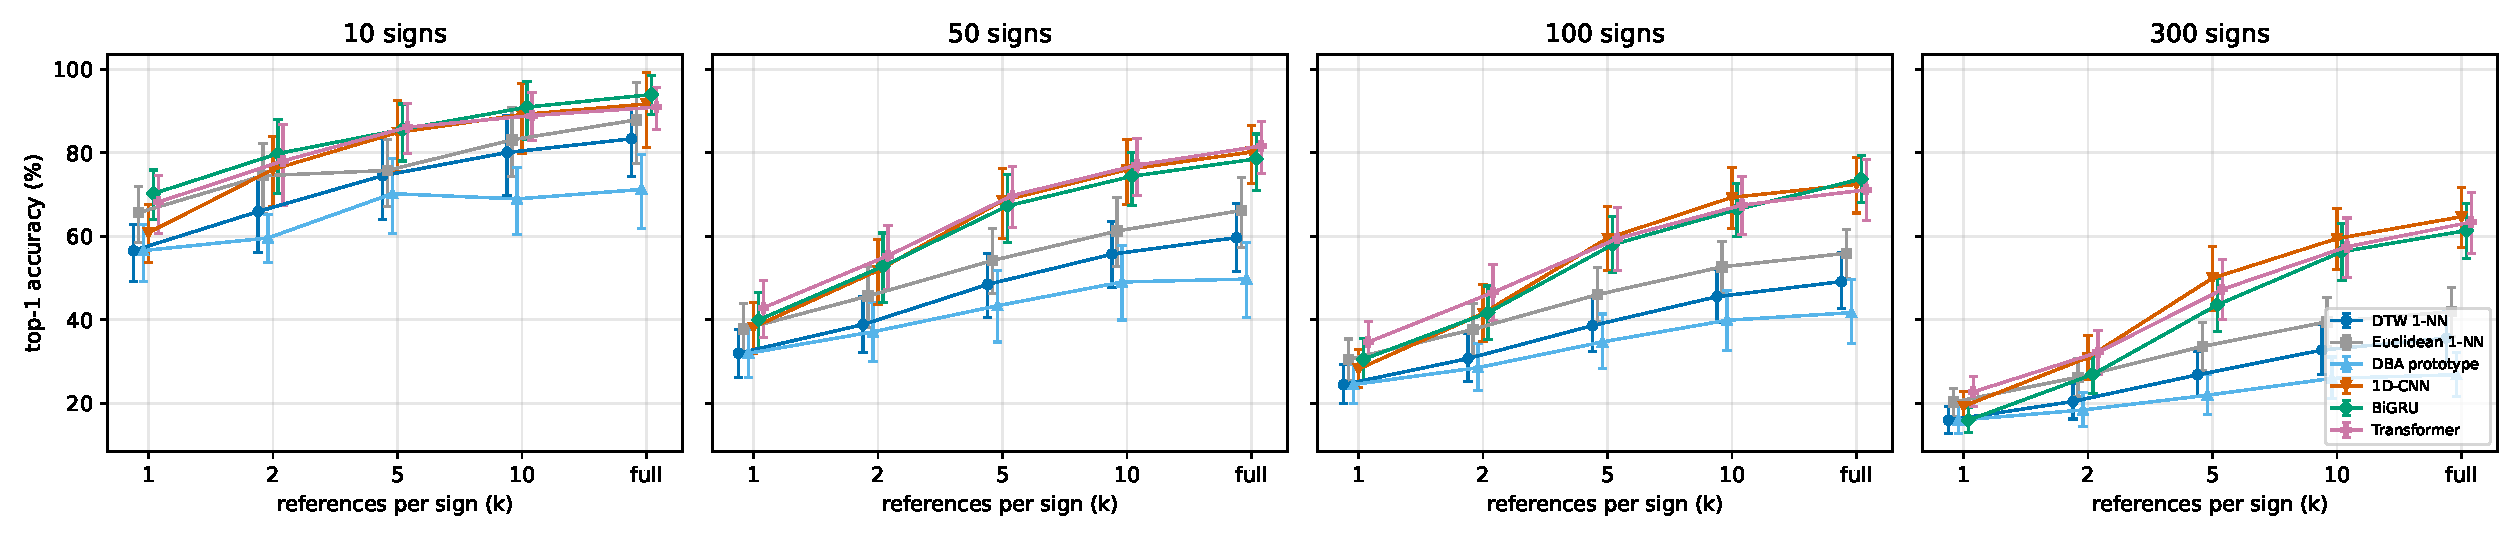
\includegraphics[width=\textwidth]{../figures_aslc/accuracy_vs_k.pdf}
\caption{ASL Citizen: top-1 accuracy versus examples per sign for vocabularies of 10, 50, 100 and 300 signs. Bars are 95\% intervals
from resampling test participants.}
\label{fig:aslc}
\end{figure*}

\paragraph{Pre-registered hypotheses.} H3: at 50 signs and $k\in\{1,2,5\}$ each learned model is above DTW. H4: at 50 signs with all training
videos at least one learned model is above DTW. \textbf{Both are supported.} \cznHOneBelowZero{} of the nine H3 comparisons have 97.5\%
intervals wholly on the learned model's side of zero (the CNN is \czdifCnnVFiftyKOne{} points above DTW at $k=1$, interval
\czdifLoCnnVFiftyKOne{} to \czdifHiCnnVFiftyKOne{}, and \czdifCnnVFiftyKFive{} points at $k=5$), and H4 holds for each model, also at the
99.17\% level adjusted for three models (\czhTwoAdjSupported). So the main PopSign finding replicates on a second dataset collected from different
signers with different devices.

\paragraph{Vocabulary size.} Accuracy falls for every method as the vocabulary grows from 10 to 300 signs, and the ordering stays the same
(Figure~\ref{fig:aslc}). With all training videos at 300 signs the CNN reaches \czaccCnnVThreeHundredKAll\%
(\czaccLoCnnVThreeHundredKAll--\czaccHiCnnVThreeHundredKAll), the Transformer \czaccTransVThreeHundredKAll\% and DTW
\czaccDtwVThreeHundredKAll\%, a CNN-minus-DTW gap of \czdifCnnVThreeHundredKAll{} points (at 10 signs: \czdifCnnVTenKAll{} points). With one
example per sign and 300 signs no method exceeds \czaccTransVThreeHundredKOne\% (Transformer).

\paragraph{Euclidean nearest neighbour versus DTW.} Euclidean 1-NN is above DTW in \cznEuclidAhead{} of the \cznEuclidCells{} (vocabulary, $k$)
cells, with the 95\% interval above zero in \cznEuclidAheadExcl{} and below zero in \cznEuclidBehindExcl{} of them. On this dataset the
extra flexibility of DTW's alignment did not help, as on PopSign (where Euclidean was above DTW in \nEuclidAhead{} of \nEuclidCells{} cells and
clearly above in \nEuclidAheadExcl{}).
